\documentclass[10pt,a4paper]{article}
\usepackage[utf8]{inputenc}
\usepackage[T1]{fontenc}
\usepackage{lmodern}
\usepackage[english]{babel}
\usepackage[margin=2.0cm]{geometry}
\usepackage{amsmath,amssymb,mathtools,bm}
\usepackage{booktabs,array,tabularx}
\newcolumntype{L}[1]{>{\raggedright\arraybackslash}p{#1}}
\usepackage{graphicx}
\usepackage{float}
\usepackage[font=small]{caption}
\usepackage{xcolor}
\usepackage{tikz}
\usetikzlibrary{arrows.meta,positioning,calc}
\usepackage[hidelinks]{hyperref}
\usepackage{url}
\makeatletter\g@addto@macro{\UrlBreaks}{\do\_\do/}\makeatother
\numberwithin{equation}{section}
\setlength{\emergencystretch}{3em}
\newcommand{\note}[1]{\begin{center}\fcolorbox{red!70!black}{red!5}{\parbox{0.94\linewidth}{\small\textbf{Note.} #1}}\end{center}}
\newcommand{\sigmaHP}{18782}
\newcommand{\sigmaStdP}{7.2\,\%}
\newcommand{\TcHP}{0.407}
\newcommand{\gKtP}{1.05}
\newcommand{\preslP}{22}
\newcommand{\costHP}{0.000304}
\newcommand{\costLinP}{0.000985}
\newcommand{\costRedP}{69}
\newcommand{\sigmaFP}{18754}
\newcommand{\TcFP}{0.407}
\newcommand{\sigmaTP}{1703}
\newcommand{\TcTP}{0.407}
\newcommand{\TsTP}{1.14}
\newcommand{\fitHP}{78 / 77 / 80}
\newcommand{\dbHP}{1.3--2.0}
\newcommand{\ArangeP}{1--3282}
\newcommand{\fitLinP}{60 / 69 / 65}
\newcommand{\sigmaHA}{1571}
\newcommand{\sigmaStdA}{1.9\,\%}
\newcommand{\TcHA}{0.232}
\newcommand{\gKtA}{0.90}
\newcommand{\preslA}{147}
\newcommand{\costHA}{0.000263}
\newcommand{\costLinA}{0.000273}
\newcommand{\costRedA}{3}
\newcommand{\sigmaFA}{1570}
\newcommand{\TcFA}{0.204}
\newcommand{\sigmaTA}{4513}
\newcommand{\TcTA}{0.232}
\newcommand{\TsTA}{7.93}
\newcommand{\fitHA}{75}
\newcommand{\dbHA}{1.6}
\newcommand{\ArangeA}{2--443}
\newcommand{\fitLinA}{75}
\newcommand{\fMassI}{56.0}
\newcommand{\fMassII}{98.2}
\newcommand{\zMassI}{0.019}
\newcommand{\zMassII}{0.031}
\newcommand{\aMassI}{$-$0.555}
\newcommand{\aMassII}{0.607}
\newcommand{\zForkA}{0.028}
\newcommand{\alphaA}{0.607}
\newcommand{\kLA}{\ensuremath{5.47\times10^{4}}}
\newcommand{\Kt}{0.258}
\newcommand{\nStartsH}{2}
\newcommand{\KppA}{7.9}
\newcommand{\KpvA}{187}
\newcommand{\KivA}{0.37}
\newcommand{\icmdMaxA}{12.2}
\newcommand{\vMaxA}{2.4}
\newcommand{\akdErrA}{302}
\newcommand{\akdErrMeasA}{1297}
\newcommand{\akdImaxA}{77}
\newcommand{\akdImaxMeasA}{10.7}
\newcommand{\clFitMinA}{96}
\newcommand{\clFitMaxA}{100}
\newcommand{\KppP}{8.0}
\newcommand{\KpvP}{53}
\newcommand{\KivP}{1.28}
\newcommand{\icmdMaxP}{5.9}
\newcommand{\vMaxP}{1.2}
\newcommand{\akdErrP}{3908}
\newcommand{\akdErrMeasP}{1316}
\newcommand{\akdImaxP}{5}
\newcommand{\akdImaxMeasP}{6.1}
\newcommand{\clFitMinP}{95}
\newcommand{\clFitMaxP}{99}


\tikzset{
  lab/.style={font=\scriptsize, inner sep=1.5pt},
  sig/.style={-{Latex[length=2mm]}, thick},
  blk/.style={draw, rounded corners, align=center, minimum height=0.9cm, fill=blue!4, font=\small},
  sum/.style={draw, circle, inner sep=1.2pt, font=\scriptsize},
}

\title{Fork modes and bearing friction of the LUCY mount:\\ modal model with Dahl bearings, identified in frequency and verified on the time-domain doublets}
\author{Generated by \texttt{build\_dahl\_report.py}\\ \small\texttt{sim/gimbal\_multidof/report\_dahl\_bearings}}
\date{\today}
\begin{document}
\maketitle

\paragraph{Purpose.} The previous model of the LUCY mount (modal least squares, fit band 1--150\,Hz; report \path{report_fork_modes}, configuration saved in \path{saved_fork_modes_modal_20261031_cad20_kt10}) represents the bearings as a linear hysteretic element $k_g(1+j\eta_g)$. That element is the equivalent linear stiffness of the bearing friction at the amplitude of the frequency-response tests. It cannot describe the doublet moves, whose amplitude is $10$ to $10^4$ times larger. This report replaces it with the Dahl friction model and verifies the result on three kinds of data:
\begin{itemize}
\item the \textbf{frequency responses} measured with WorkBench (fit band 1--150\,Hz);
\item the \textbf{doublets} ($+A$, $-2A$, $+A$ from 0.1 to 8$^\circ$) driven in \textbf{open loop} by the measured motor current;
\item the same doublets in \textbf{closed loop}: the measured position reference enters the model of the AKD2G drive, and the current is produced by the control loops.
\end{itemize}

\paragraph{Main results.}
\begin{itemize}
\item \textbf{Hybrid identification of the bearings.} The doublets measure the sliding level $T_c$ of the friction; the frequency responses measure the pre-sliding stiffness $\sigma_0$. The bearing parameters are therefore taken from the data that determine them: $T_c$ from the doublets and $\sigma_0$ from the frequency responses, the latter estimated together with the structure.
  \begin{itemize}
  \item Azimuth: $T_c=\TcHA$\,N\,m, $\sigma_0=\sigmaHA$\,N\,m/rad (std \sigmaStdA), pre-sliding scale $T_c/\sigma_0=\preslA\,\mu$rad.
  \item Elevation: $T_c=\TcHP$\,N\,m, $\sigma_0=\sigmaHP$\,N\,m/rad (std \sigmaStdP), pre-sliding scale $\preslP\,\mu$rad.
  \end{itemize}
\item \textbf{Frequency domain.} The fit of the elevation goes from \fitLinP\,\% to \fitHP\,\% on the three measurements, and its cost falls by \costRedP\,\%. In azimuth the fit stays at \fitHA\,\% with a lower rms magnitude error (\dbHA\,dB against 2.5\,dB), and the antiresonance near 12\,Hz is placed where it is measured.
\item \textbf{Time domain, open loop} (measured current in). The beginning of each move is reproduced, but the model drifts at rest: the holding torque measured at rest exceeds $T_c$, and the pure Dahl element cannot hold it. In azimuth the model is also about 20\,\% short of torque, a figure that depends on the undocumented scale of the current channel.
\item \textbf{Time domain, closed loop} (measured reference in). With the effective gains of the position and velocity loops, estimated on the 1$^\circ$ doublet, the model reproduces the position of all the moves from 0.5 to 8$^\circ$ with fit \clFitMinA--\clFitMaxA\,\% in azimuth and \clFitMinP--\clFitMaxP\,\% in elevation. The current peaks agree within 10--15\,\%. Two features are not reproduced: an oscillation of the azimuth current near 7\,Hz, and the stick-slip behaviour at very small moves and at rest.
\end{itemize}

\note{The H7 configuration still contains placeholder data (inertias of the encoder and motor nodes, materials); the figures carry the label ``result from placeholder parameters''. The motor current of the doublets is the PLC channel \texttt{AXIS*\_AMPS}, taken as $2I_\mathrm{rms}$ as in \path{closedLoopModel}; that scale is not documented (Section~\ref{sec:limits}).}

\tableofcontents

%% ===================================================================================================
\section{Data}\label{sec:data}
\paragraph{Frequency responses.} The four WorkBench ``Plant'' responses of 28/10/2026 used by the previous model, encoder velocity over motor current in (rad/s)/A$_\mathrm{rms}$:
\begin{itemize}
\item elevation: 1--600\,Hz on a 1\,\% grid, 30--150\,Hz on a 1\,\% grid, and 30--300\,Hz with 16 ring screws at 4\,A;
\item azimuth: 1--600\,Hz on a 3\,\% grid, 3.5\,A.
\end{itemize}
Only the points between 1 and 150\,Hz are fitted. The exports also contain the controller and open-loop traces; the open loop is used here to compute the motion of the bearings during the tests (Section~\ref{sec:df}).

\paragraph{Doublets.} \path{LucyIdentification/VClosedLoop/V2}, recorded on 20/10/2026 by the PLC at 2\,kHz: one axis per file, three moves $+A$, $-2A$, $+A$ at 10$^\circ$/s with rests of about 35\,s. Amplitudes used: 0.1, 0.5, 1, 3, 5 and 8$^\circ$ on each axis, i.e.\ 18 moves per axis. Channels: position reference and encoder position (millidegrees), and motor current \texttt{AXIS*\_AMPS} (\texttt{AXIS1} azimuth, \texttt{AXIS2} elevation). Each move is a window from 0.5\,s before the reference starts to 12\,s after it, or to the next move.

\paragraph{Drives.} \path{Parameters_azimuth.akd} and \path{Parameters_elevation.akd}, with gains and filters of the WorkBench exports of the same session (\path{V2/BodeMeasurement_*.csv}).

%% ===================================================================================================
\section{Model}\label{sec:model}
\subsection{Structure in modal form}
Each axis is the lumped model of the previous report: elevation with the telescope rigid on the ring and two modal masses on the motor stator, azimuth with the load split into fork base and fork top. The bearings are removed from the stiffness:
\begin{equation}
\mathbf M\ddot{\mathbf x}+\mathbf C\dot{\mathbf x}+\mathbf K_0\mathbf x=\mathbf e\,\tau_m-\mathbf v\,T_b,\qquad \theta_\mathrm{enc}=\mathbf c^T\mathbf x,\qquad \delta=\mathbf v^T\mathbf x .\label{eq:struct}
\end{equation}
\begin{itemize}
\item $\tau_m$ is the motor torque. $\mathbf e$ applies it to the rotor and, in elevation, its reaction to the stator modal masses.
\item $\delta$ is the bearing deflection: hub minus stator structure in elevation, fork base minus ground in azimuth. $T_b$ is the friction torque that the bearings transmit.
\item The modes of $(\mathbf M,\mathbf K_0)$, $\mathbf K_0\bm\phi_k=\omega_k^2\mathbf M\bm\phi_k$ with $\bm\Phi^T\mathbf M\bm\Phi=\mathbf I$, now include the rigid rotation of the axis ($\omega_1\simeq0$). Each mode has its own viscous modal damping, so that $\mathbf C=\mathbf M\bm\Phi\,\mathrm{diag}(2\zeta_k\omega_k)\,\bm\Phi^T\mathbf M$.
\end{itemize}

\subsection{Dahl friction in the bearings}
The bearings are a Dahl element acting on $\delta$. Its internal state $z$ is the mean deflection of the contact asperities (the ``bristles''):
\begin{equation}
\frac{dz}{dt}=\dot\delta-\frac{\sigma_0\,|\dot\delta|}{T_c}\,z,\qquad T_b=\sigma_0 z .\label{eq:dahl}
\end{equation}
\begin{itemize}
\item \textbf{Pre-sliding.} For small motion, $|\sigma_0 z|\ll T_c$, the element is a spring of stiffness $\sigma_0$.
\item \textbf{Sliding.} For motion well beyond the pre-sliding scale $T_c/\sigma_0$, $T_b\to T_c\,\mathrm{sign}(\dot\delta)$: Coulomb friction.
\item The transition between the two regimes is smooth and hysteretic. The dissipation per cycle depends on the amplitude, not on the frequency.
\end{itemize}
The Dahl model is the LuGre model with static torque equal to the Coulomb torque ($T_s=T_c$) and no micro-damping or viscous term ($\sigma_1=\sigma_2=0$). LuGre with all six parameters was also identified; it fits the frequency responses only slightly better and its parameters are not identifiable (Section~\ref{sec:res_freq}).

\subsection{Frequency domain: describing function}\label{sec:df}
\paragraph{Describing function.} Under a sinusoidal deflection $\delta=A\sin\omega t$, the first harmonic of $T_b$ defines a complex, amplitude-dependent bearing stiffness:
\begin{equation}
K_b(A,\omega)=\frac{\frac{1}{\pi}\int_0^{2\pi}T_b(\varphi)\,e^{-j\varphi}\,d\varphi}{-jA},\qquad \varphi=\omega t .\label{eq:df}
\end{equation}
It is computed by integrating~\eqref{eq:dahl} over three cycles, 256 steps per cycle, with the exact update of $z$ at constant velocity over each step, and taking the last cycle. Its limits are:
\begin{equation}
K_b\to\sigma_0\quad\bigl(A\ll T_c/\sigma_0\bigr),\qquad K_b\to j\,\frac{4T_c}{\pi A}\quad\bigl(A\gg T_c/\sigma_0\bigr).
\end{equation}
The linear hysteretic element of the previous model, $k_g(1+j\eta_g)$, is one value of $K_b$ at one amplitude.

\paragraph{Plant.} The bearings act on the single deflection $\delta=\mathbf w^T\mathbf z$, with $\mathbf w=\bm\Phi^T\mathbf v$, and enter the modal superposition as an exact rank-one term (Sherman--Morrison). With $D_k=s^2+2\zeta_k\omega_ks+\omega_k^2$, $\mathbf b=\bm\Phi^T\mathbf e$, $\mathbf g=\bm\Phi^T\mathbf c$ and $h=K_b(A,\omega)$:
\begin{equation}
G_\theta=\sum_k\frac{g_kb_k}{D_k}-\frac{h\Bigl(\sum_k\dfrac{g_kw_k}{D_k}\Bigr)\Bigl(\sum_k\dfrac{w_kb_k}{D_k}\Bigr)}{1+h\displaystyle\sum_k\frac{w_k^2}{D_k}},\qquad
G(s)=s\,g_{K_t}K_t\,G_\theta(s)\,\frac{\omega_i}{s+\omega_i}\,e^{-s\tau_d}, \label{eq:plant}
\end{equation}
\begin{itemize}
\item $K_t=\Kt$\,N\,m/A$_\mathrm{rms}$ is the catalogue torque constant of the TBM(S)-7646-A at 25\,$^\circ$C, and $g_{K_t}$ its tolerance factor;
\item $\omega_i/(s+\omega_i)$ is the current loop (1.5\,kHz), and $\tau_d$ an equivalent delay.
\end{itemize}

\paragraph{Amplitude of the bearings.} The tests are run in closed loop: WorkBench injects $I_\mathrm{exc}$ at the current command while the position and velocity loops are active, so that the motor carries $I_\mathrm{exc}S$ with $S=1/(1+L)$. Below the fork modes the stator barely moves and the encoder reads the bearing deflection, so its amplitude follows from the measured traces:
\begin{equation}
A(\omega)=\frac{|G_\mathrm{mis}(j\omega)|\,I_\mathrm{exc}\,|S_\mathrm{mis}(j\omega)|}{\omega},\qquad S_\mathrm{mis}=\frac{1}{1+L_\mathrm{mis}} .\label{eq:amp}
\end{equation}
During the frequency responses the bearing amplitude ranges over \ArangeA\,$\mu$rad in azimuth and \ArangeP\,$\mu$rad in elevation (Figure~\ref{fig:df_amp}), across the pre-sliding scale. The amplitude is taken from the measurement for each measurement and frequency. This introduces a partial circularity, discussed in Section~\ref{sec:limits}.

\subsection{Time domain, open loop: measured current in}\label{sec:ol}
The current $i$ measured during the doublets drives the structure, $\tau_m=g_{K_t}K_t\,i$, with $i=\texttt{AMPS}/2$ filtered at 150\,Hz. With the state $\mathbf s=[\mathbf x;\dot{\mathbf x}]$, the linear part of~\eqref{eq:struct} is discretised exactly with step $\Delta t=0.5$\,ms (zero-order hold of $\tau_m$ and $T_b$):
\begin{equation}
\mathbf s_{k+1}=\mathbf A_d\mathbf s_k+\mathbf B_d\begin{bmatrix}\tau_{m,k}\\ T_{b,k}\end{bmatrix},\qquad \mathbf A_d=e^{\mathbf A\Delta t},\quad \mathbf B_d=\int_0^{\Delta t}e^{\mathbf A t}\,dt\,\mathbf B .
\end{equation}
The Dahl state is advanced exactly at the mean bearing velocity $\bar{\dot\delta}$ of the step:
\begin{equation}
z_{k+1}=z_k\,e^{-a\Delta t}+\frac{\bar{\dot\delta}}{a}\bigl(1-e^{-a\Delta t}\bigr),\qquad a=\frac{\sigma_0|\bar{\dot\delta}|}{T_c} .\label{eq:zupdate}
\end{equation}
\paragraph{Initial condition.} At rest the friction holds the measured holding torque; it is limited to $T_c$, the largest torque a Dahl element can hold.

\subsection{Time domain, closed loop: position reference in}\label{sec:cl}
The measured position reference $p_\mathrm{cmd}$ drives the model of the AKD2G drive of \path{closedLoopModel/lucy_cl}, which gives the motor voltage; the current follows from the motor electrical equation (Figure~\ref{fig:cl}):
\begin{gather}
v_\mathrm{cmd}=K_{pp}(p_\mathrm{cmd}-\theta_\mathrm{enc}),\qquad
i_\mathrm{cmd}=K_{pv}\Bigl(1+\frac{2\pi K_{iv}}{s}\Bigr)H_\mathrm{fwd}(s)\bigl(v_\mathrm{cmd}-H_\mathrm{fb}(s)\,\dot\theta_\mathrm{enc}\bigr),\\
u=K_{pi}\Bigl(1+\frac{R}{Ls}\Bigr)(i_\mathrm{cmd}-i),\qquad L_\mathrm{ph}\frac{di}{dt}=\frac u2-R_\mathrm{ph}\,i-K_{e,\mathrm{ph}}\,\omega_r,\qquad \tau_m=g_{K_t}K_t\,i-b\,\omega_r .\label{eq:drive}
\end{gather}
\begin{itemize}
\item $H_\mathrm{fwd}$ and $H_\mathrm{fb}$ are the biquad filters of the drive (and the observer in elevation), from the WorkBench exports of the V2 session.
\item The current PI has its zero on the electrical pole $R/L$, which gives a 1.5\,kHz current loop. Motor data are those of the TBM(S)-7646-A datasheet; $\omega_r=\mathbf e^T\dot{\mathbf x}$ is the rotor speed relative to the stator.
\end{itemize}
Below the limits of the drive (current 18\,A, velocity integrator, phase voltage) the drive is linear. Its matrices are taken from \texttt{Drive.step} of \path{lucy_cl}. Structure, motor and drive are discretised together exactly, with step 0.1\,ms and inputs $p_\mathrm{cmd}$ and $T_b$; the Dahl state is updated with~\eqref{eq:zupdate}. The largest current command in the simulations is \icmdMaxA\,A in azimuth and \icmdMaxP\,A in elevation, so the limits are never reached. The initial state is the equilibrium of the loop with the friction holding the measured holding torque (limited to $T_c$).

\begin{figure}[H]\centering
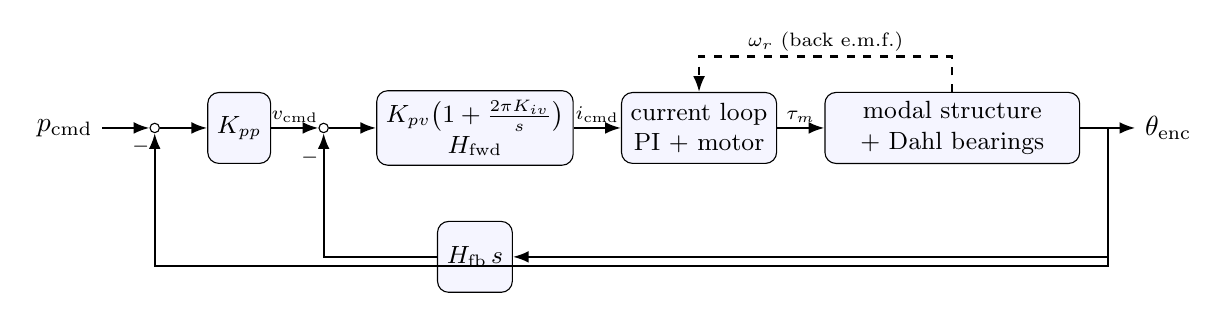
\begin{tikzpicture}[node distance=6mm]
\node (p) {$p_\mathrm{cmd}$};
\node[sum, right=of p] (s1) {};
\node[blk, right=of s1] (kp) {$K_{pp}$};
\node[sum, right=of kp] (s2) {};
\node[blk, right=of s2] (cv) {$K_{pv}\bigl(1+\frac{2\pi K_{iv}}{s}\bigr)$\\ $H_\mathrm{fwd}$};
\node[blk, right=of cv] (ci) {current loop\\ PI + motor};
\node[blk, right=of ci, text width=3.0cm] (pl) {modal structure\\ + Dahl bearings};
\node[right=7mm of pl] (y) {$\theta_\mathrm{enc}$};
\node[blk, below=7mm of cv] (hf) {$H_\mathrm{fb}\,s$};
\draw[sig] (p) -- (s1); \draw[sig] (s1) -- (kp); \draw[sig] (kp) -- node[above, lab]{$v_\mathrm{cmd}$} (s2);
\draw[sig] (s2) -- (cv); \draw[sig] (cv) -- node[above, lab]{$i_\mathrm{cmd}$} (ci);
\draw[sig] (ci) -- node[above, lab]{$\tau_m$} (pl); \draw[sig] (pl) -- (y);
\draw[sig] ($(pl.east)!0.5!(y.west)$) |- (hf.east); \draw[sig] (hf.west) -| node[pos=0.9, left, lab]{$-$} (s2.south);
\draw[sig] ($(pl.east)!0.5!(y.west)$) -- ++(0,-1.75) -| node[pos=0.95, left, lab]{$-$} (s1.south);
\draw[sig, dashed] (pl.north) -- ++(0,0.45) -| node[pos=0.25, above, lab]{$\omega_r$ (back e.m.f.)} (ci.north);
\end{tikzpicture}
\caption{Closed loop of one axis (Section~\ref{sec:cl}). In open loop (Section~\ref{sec:ol}) the measured current replaces the drive and the motor: $\tau_m=g_{K_t}K_t\,i$.}\label{fig:cl}
\end{figure}

%% ===================================================================================================
\section{Identification}\label{sec:ident}
\subsection{Cost and constraints}
The cost is the one of the previous model: the squared differences of the real and imaginary parts of the plant over the measured points in 1--150\,Hz, each weighted by the width in $\ln f$ that the point represents,
\begin{equation}
F(\mathbf p)=\frac12\sum_i w_i^2\,\bigl|G(j\omega_i;\mathbf p,A_i)-G_\mathrm{mis}(j\omega_i)\bigr|^2,\qquad w_i=\sqrt{\Delta\ln f_i/0.01},
\end{equation}
where $A_i$ is the bearing amplitude~\eqref{eq:amp} of the measurement the point belongs to. The constraints are those of the saved configuration:
\begin{itemize}
\item modal damping $\zeta_k\leq0.05$;
\item CAD inertias and stiffnesses within $\pm20$\,\%;
\item torque-constant factor $g_{K_t}\in[0.9,1.1]$ per axis (catalogue tolerance);
\item the stiffness introduced between fork base and fork top, and the stator masses (frequency and residue), free;
\item telescope rigid on the ring.
\end{itemize}
The bearing parameters $k_g$, $\eta_g$ of the previous model are replaced by those of the friction. The solver is the bounded trust-region least squares of SciPy, with several starts and the covariance computed on the parameters not at a bound.

\subsection{Hybrid identification of the bearings}
Two independent identifications of the Dahl parameters exist:
\begin{itemize}
\item \textbf{in the time domain}, on the doublets (\path{closedLoopModel/results_v2_identification}, with Stribeck curve $T_s/T_c$);
\item \textbf{in frequency}, on the responses of Section~\ref{sec:data} ($\sigma_0$, $T_c$ and the structure together).
\end{itemize}
They agree on $T_c$ and disagree on $\sigma_0$ by a factor 3 to 11 (Table~\ref{tab:friction}). The reason is what each set of data contains:
\begin{itemize}
\item The doublets move the axis by 1.7 to 280\,mrad: they are almost entirely in sliding, and determine $T_c$. In the time-domain identification $\sigma_0$ was not estimated but fixed in the selection of the structure.
\item The frequency responses move the bearings by 1 to 3300\,$\mu$rad, across the pre-sliding scale, and determine $\sigma_0$. In azimuth they determine both parameters (std 2 and 4\,\%); in elevation $\sigma_0$, $T_c$ and $g_{K_t}$ are not separable (their standard deviations are not defined).
\end{itemize}
The \textbf{hybrid identification} therefore fixes $T_c$ at the time-domain value and estimates $\sigma_0$ together with the structure on the frequency responses, with the constraints above and a pure Dahl element ($T_s=T_c$). The high static torque of the time-domain azimuth model ($T_s=\TsTA\,T_c$) is not compatible with the frequency responses (Section~\ref{sec:res_freq}). Two starts were used per axis, from $\sigma_0$ of each domain; both reach the same minimum. With $T_c$ fixed, $\sigma_0$ becomes identifiable on both axes.

\begin{table}[H]\centering\footnotesize\setlength{\tabcolsep}{4pt}
\caption{Dahl parameters of the bearings. Std: relative standard deviation (``n.d.'': not determined by the data). Pre-sliding scale: $T_c/\sigma_0$.}\label{tab:friction}
\begin{tabular}{llrrrrrr}\toprule
axis & source & $\sigma_0$ [N\,m/rad] & std & $T_c$ [N\,m] & std & $T_s/T_c$ & $T_c/\sigma_0$ [$\mu$rad] \\ \midrule
azimuth & doublets (V2, time domain) & 4513 & -- & 0.232 & -- & 7.93 & 51 \\
 & FRF (frequency domain) & 1570 & 2.1\,\% & 0.204 & 4.0\,\% & 1 & 130 \\
 & \textbf{hybrid} & \textbf{1571} & 1.9\,\% & \textbf{0.232} (fixed) & -- & 1 & 147 \\
elevation & doublets (V2, time domain) & 1703 & -- & 0.407 & -- & 1.14 & 239 \\
 & FRF (frequency domain) & \ensuremath{1.875\times10^{4}} & n.d. & 0.407 & n.d. & 1 & 22 \\
 & \textbf{hybrid} & \textbf{\ensuremath{1.878\times10^{4}}} & 7.2\,\% & \textbf{0.407} (fixed) & -- & 1 & 22
\\ \bottomrule
\end{tabular}\end{table}

%% ===================================================================================================
\section{Results: frequency domain}\label{sec:res_freq}
\begin{table}[H]\centering\footnotesize\setlength{\tabcolsep}{4pt}
\caption{Elevation, fit band 1--150\,Hz: cost, NRMSE fit on the three measurements (1--600\,Hz / 30--150\,Hz / 16 screws), fit in 1--5\,Hz, and rms magnitude and phase errors.}\label{tab:freq_el}
\begin{tabular}{L{6.2cm}rrrrr}\toprule
bearing model & cost & fit [\%] & 1--5\,Hz [\%] & rms [dB] & rms [deg] \\ \midrule
linear hysteretic $k_g(1+j\eta_g)$ (previous model) & 0.000985 & 60 / 69 / 65 & 67 & 2.1--2.7 & 8--18 \\
LuGre, all 6 parameters from the FRF & 0.000272 & 79 / 77 / 81 & 87 & 1.2--1.9 & 7--8 \\
Dahl, $\sigma_0$ and $T_c$ from the FRF & 0.000304 & 78 / 77 / 80 & 82 & 1.3--2.0 & 6--9 \\
\textbf{Dahl hybrid}: $T_c$ doublets, $\sigma_0$ FRF & 0.000304 & 78 / 77 / 80 & 82 & 1.3--2.0 & 6--9 \\
Dahl from the doublets, same structure & 0.00297 & 29 / 35 / 70 & 45 & 2.2--3.3 & 8--17 \\
Dahl from the doublets, structure refitted & 0.00129 & 53 / 68 / 65 & 60 & 2.4--3.0 & 9--17
\\ \bottomrule
\end{tabular}\end{table}

\begin{table}[H]\centering\footnotesize\setlength{\tabcolsep}{4pt}
\caption{Azimuth, fit band 1--150\,Hz: as Table~\ref{tab:freq_el}, one measurement.}\label{tab:freq_az}
\begin{tabular}{L{6.2cm}rrrrr}\toprule
bearing model & cost & fit [\%] & 1--5\,Hz [\%] & rms [dB] & rms [deg] \\ \midrule
linear hysteretic $k_g(1+j\eta_g)$ (previous model) & 0.000273 & 75 & 89 & 2.5 & 17 \\
LuGre, all 6 parameters from the FRF & 0.000242 & 76 & 94 & 3.2 & 18 \\
Dahl, $\sigma_0$ and $T_c$ from the FRF & 0.000257 & 76 & 90 & 2.2 & 9 \\
\textbf{Dahl hybrid}: $T_c$ doublets, $\sigma_0$ FRF & 0.000263 & 75 & 90 & 1.6 & 15 \\
Dahl from the doublets, same structure & 0.00282 & 19 & $-$36 & 7.2 & 42 \\
Dahl from the doublets, structure refitted & 0.0027 & 21 & $-$35 & 6.5 & 37
\\ \bottomrule
\end{tabular}\end{table}

\paragraph{Elevation} (Table~\ref{tab:freq_el}, Figure~\ref{fig:freq_el}).
\begin{itemize}
\item \textbf{Fit.} The hybrid Dahl model lowers the cost from \costLinP\ to \costHP\ ($-$\costRedP\,\%) and reproduces the low-frequency shape between the bearing mode and 30\,Hz, and partly reproduces the features at 6--9\,Hz, which no linear model reproduced.
\item \textbf{Equivalence of the Dahl variants.} In elevation $T_c$ from the doublets equals the value fitted in frequency, so the hybrid and the frequency-only Dahl models coincide; fixing $T_c$ only makes $\sigma_0$ identifiable.
\item \textbf{Stator masses.} \fMassI\ and \fMassII\,Hz, with damping \zMassI\ and \zMassII\ and residues \aMassI\ and \aMassII\,(kg\,m$^2$)$^{-1}$. The torque factor is $g_{K_t}=\gKtP$.
\end{itemize}

\paragraph{Azimuth} (Table~\ref{tab:freq_az}, Figure~\ref{fig:freq_az}).
\begin{itemize}
\item \textbf{Fit.} The cost is close to that of the linear model, and the rms magnitude error is the lowest of all variants (\dbHA\,dB). The antiresonance near 12\,Hz is placed within about 0.1\,Hz of the measured one, where the linear model put it about 0.6\,Hz low.
\item \textbf{Parameters.} The fork mode keeps $\zeta=\zForkA$, $\alpha=\alphaA$ and $k_{LA}=$\,\kLA\,N\,m/rad. The torque factor stays at its lower bound, $g_{K_t}=\gKtA$.
\end{itemize}

\paragraph{The other bearing models.}
\begin{itemize}
\item \textbf{Time-domain Dahl parameters.} Used directly, they spoil both axes, even with the structure refitted: fit 19--21\,\% in azimuth. In azimuth $\sigma_0$ is about 3 times larger and $T_s=\TsTA\,T_c$: at the amplitudes of the frequency responses the bearing stays in pre-sliding, stiff and lightly dissipative, and the bearing mode moves from 3 to about 5\,Hz. In elevation the describing functions of the two domains coincide below 6\,Hz, where the bearing slides and only $T_c$ matters, and differ above (Figure~\ref{fig:df_tf}).
\item \textbf{LuGre.} With all six parameters it fits slightly better than Dahl, but $T_s/T_c$ and $\sigma_1$ go to their bounds and $\sigma_0$, $T_c$, $\sigma_2$, $g_{K_t}$ are not identifiable in elevation. Dahl is preferred: two parameters, both identified.
\end{itemize}

\begin{figure}[H]\centering
\includegraphics[width=0.94\linewidth]{figures/freq_elevation.pdf}
\caption{Elevation plant [dB (rad/s)/A] and phase: measurements and models with the Dahl bearings (frequency-domain fit, hybrid, time-domain parameters with the structure refitted) and the previous linear hysteretic model.}\label{fig:freq_el}
\end{figure}

\begin{figure}[H]\centering
\includegraphics[width=0.94\linewidth]{figures/freq_azimuth.pdf}
\caption{Azimuth plant and phase: as Figure~\ref{fig:freq_el}.}\label{fig:freq_az}
\end{figure}

\begin{figure}[H]\centering
\includegraphics[width=0.95\linewidth]{figures/df_time_vs_freq.pdf}
\caption{Describing function of the bearings at the measured amplitude (first measurement of each axis): magnitude and loss factor, for $\sigma_0$ and $T_c$ of the frequency-domain fit, of the hybrid identification and of the time-domain identification.}\label{fig:df_tf}
\end{figure}

\begin{figure}[H]\centering
\includegraphics[width=0.95\linewidth]{figures/df_amplitude.pdf}
\caption{Frequency-domain Dahl fit: describing function and bearing amplitude~\eqref{eq:amp} for each measurement, against the pre-sliding scale $T_c/\sigma_0$.}\label{fig:df_amp}
\end{figure}

\begin{table}[H]\centering\scriptsize\setlength{\tabcolsep}{3pt}
\caption{Hybrid model, elevation: parameters. Std: relative standard deviation of the free parameters.}\label{tab:hyb_el}
\begin{tabular}{lL{2.4cm}lrlrl}\toprule
param. & class & unit & estimate & bounds & std & at bound \\ \midrule
$s_{J_e}$ & CAD, $\pm20$\,\% & -- & 0.8585 & [0.8, 1.2] & n.d. &  \\
$s_{J_{hp}}$ & CAD, $\pm20$\,\% & -- & 0.9979 & [0.8, 1.2] & 1.2\,\% &  \\
$s_{J_m}$ & CAD, $\pm20$\,\% & -- & 0.8 & [0.8, 1.2] & -- & yes \\
$s_{J_\mathrm{rear}}$ & CAD, $\pm20$\,\% & -- & 0.8 & [0.8, 1.2] & -- & yes \\
$s_{k_{\theta1}}$ & CAD, $\pm20$\,\% & -- & 0.9155 & [0.8, 1.2] & n.d. &  \\
$s_{k_{\theta2}}$ & CAD, $\pm20$\,\% & -- & 1.2 & [0.8, 1.2] & -- & yes \\
$s_{k_{\theta3}}$ & CAD, $\pm20$\,\% & -- & 0.9138 & [0.8, 1.2] & n.d. &  \\
$\sigma_0$ & bearings, free & N\,m/rad & \ensuremath{1.878\times10^{4}} & [10, \ensuremath{1\times10^{7}}] & 7.2\,\% &  \\
$T_c$ & bearings, doublets & N\,m & 0.4073 & fixed & -- &  \\
$\tau_d$ & drive & s & 0.0004709 & [\ensuremath{1\times10^{-6}}, 0.002] & 9.4\,\% &  \\
$f_1$ & stator mass, free & Hz & 56 & [40, 80] & 0.1\,\% &  \\
$a_1$ & stator mass, free & (kg\,m$^2$)$^{-1}$ & $-$0.5549 & [$-$50, 50] & 2.9\,\% &  \\
$f_2$ & stator mass, free & Hz & 98.24 & [80, 140] & 0.2\,\% &  \\
$a_2$ & stator mass, free & (kg\,m$^2$)$^{-1}$ & 0.6066 & [$-$50, 50] & 4.4\,\% &  \\
$g_{K_t}$ & motor, $\pm10$\,\% & -- & 1.05 & [0.9, 1.1] & 0.7\,\% &  \\
$\zeta_2$ & modal, $\leq0.05$ & -- & 0.01922 & [0.0001, 0.05] & 5.8\,\% &  \\
$\zeta_3$ & modal, $\leq0.05$ & -- & 0.0309 & [0.0001, 0.05] & 6.4\,\% &  \\
$\zeta_4$ & modal, $\leq0.05$ & -- & 0.0001 & [0.0001, 0.05] & -- & yes \\
$\zeta_5$ & modal, $\leq0.05$ & -- & 0.0001 & [0.0001, 0.05] & -- & yes \\
$\zeta_6$ & modal, $\leq0.05$ & -- & 0.0001969 & [0.0001, 0.05] & n.d. & 
\\ \bottomrule
\end{tabular}\end{table}

\begin{table}[H]\centering\scriptsize\setlength{\tabcolsep}{3pt}
\caption{Hybrid model, azimuth: parameters.}\label{tab:hyb_az}
\begin{tabular}{lL{2.4cm}lrlrl}\toprule
param. & class & unit & estimate & bounds & std & at bound \\ \midrule
$s_{J_e}$ & CAD, $\pm20$\,\% & -- & 0.8 & [0.8, 1.2] & -- & yes \\
$s_{J_m}$ & CAD, $\pm20$\,\% & -- & 0.8 & [0.8, 1.2] & -- & yes \\
$s_{J_L}$ & CAD, $\pm20$\,\% & -- & 1.135 & [0.8, 1.2] & 1.2\,\% &  \\
$s_{k_1}$ & CAD, $\pm20$\,\% & -- & 1.2 & [0.8, 1.2] & -- & yes \\
$s_{k_2}$ & CAD, $\pm20$\,\% & -- & 1.2 & [0.8, 1.2] & -- & yes \\
$\alpha$ & introduced, free & -- & 0.6066 & [0.02, 0.98] & 2.1\,\% &  \\
$k_{LA}$ & introduced, free & N\,m/rad & \ensuremath{5.474\times10^{4}} & [\ensuremath{1\times10^{3}}, \ensuremath{1\times10^{8}}] & 2.3\,\% &  \\
$\sigma_0$ & bearings, free & N\,m/rad & 1571 & [10, \ensuremath{1\times10^{7}}] & 1.9\,\% &  \\
$T_c$ & bearings, doublets & N\,m & 0.2316 & fixed & -- &  \\
$\tau_d$ & drive & s & 0.0004781 & [\ensuremath{1\times10^{-6}}, 0.002] & 4.2\,\% &  \\
$g_{K_t}$ & motor, $\pm10$\,\% & -- & 0.9 & [0.9, 1.1] & -- & yes \\
$\zeta_2$ & modal, $\leq0.05$ & -- & 0.02818 & [0.0001, 0.05] & 6.0\,\% &  \\
$\zeta_3$ & modal, $\leq0.05$ & -- & 0.0001 & [0.0001, 0.05] & -- & yes \\
$\zeta_4$ & modal, $\leq0.05$ & -- & 0.05 & [0.0001, 0.05] & -- & yes
\\ \bottomrule
\end{tabular}\end{table}

%% ===================================================================================================
\section{Results: doublets in open loop (measured current in)}\label{sec:res_ol}
The hybrid model is driven by the measured current, with no parameter estimated on these data. Table~\ref{tab:ol} gives the position fit during each move, from the start of the reference to 0.5\,s after its end.

\begin{table}[H]\centering\footnotesize
\caption{Open loop: NRMSE fit [\%] of the encoder position during the three moves of each doublet.}\label{tab:ol}
\begin{tabular}{lll}\toprule
amplitude [$^\circ$] & azimuth & elevation \\ \midrule
0.1 & $-$1532 / $-$13 / $-$149 & 36 / $-$64 / $-$54 \\
0.5 & 33 / 44 / 86 & 22 / 10 / 22 \\
1 & 64 / 49 / 59 & 43 / $-$54 / 58 \\
3 & 82 / 42 / 31 & 4 / $-$34 / 58 \\
5 & 75 / 54 / 27 & 37 / $-$34 / 37 \\
8 & $-$40 / 23 / 23 & 17 / $-$83 / 6
\\ \bottomrule
\end{tabular}\end{table}

\begin{itemize}
\item \textbf{Start of the moves.} The acceleration, the oscillation of about 7\,Hz imposed by the controller, and the braking are reproduced at the start of every move (Figures~\ref{fig:ol_az}, \ref{fig:ol_el}). In elevation the peak velocity of the 1$^\circ$ move is also right in amplitude.
\item \textbf{Drift at rest.} At rest the real axis holds torques above $T_c$: about 0.29\,N\,m in azimuth before the 0.1$^\circ$ move, and about 0.54\,N\,m in elevation after the 1$^\circ$ move. A pure Dahl element cannot exceed $T_c$, so the model slides and drifts quadratically, by up to tens of degrees.
\item \textbf{Torque in azimuth.} The model is short of torque by about 20\,\%: peak velocity 0.065 against 0.080\,rad/s at 1$^\circ$, cruise velocity 0.125 against 0.175\,rad/s at 5$^\circ$. With \texttt{AMPS}~$=2I_\mathrm{rms}$, the doublets ask for about 1.26 times the torque per ampere given by the frequency responses. The scale of the current channel is not documented (Section~\ref{sec:limits}).
\item \textbf{Why open loop is ill conditioned.} A current-driven axis integrates any torque error twice. The open-loop test is therefore sensitive to the holding torques and to the current scale, not only to the plant.
\end{itemize}

\begin{figure}[H]\centering
\includegraphics[width=\linewidth]{figures/ol_azimuth.pdf}
\caption{Azimuth, open loop: encoder position, velocity and input current for one move of the 0.1, 1 and 5$^\circ$ doublets; measurement and hybrid model.}\label{fig:ol_az}
\end{figure}

\begin{figure}[H]\centering
\includegraphics[width=\linewidth]{figures/ol_elevation.pdf}
\caption{Elevation, open loop: as Figure~\ref{fig:ol_az}.}\label{fig:ol_el}
\end{figure}

%% ===================================================================================================
\section{Results: doublets in closed loop (position reference in)}\label{sec:res_cl}
\paragraph{Gains of the drives.} With the gains of the \texttt{.akd} files and of the WorkBench exports, the model does not reproduce the doublets:
\begin{itemize}
\item azimuth: largest following error \akdErrA\,mdeg against \akdErrMeasA\,mdeg measured, and current command up to \akdImaxA\,A (unsaturated model) against \akdImaxMeasA\,A measured;
\item elevation: largest following error \akdErrP\,mdeg against \akdErrMeasP\,mdeg.
\end{itemize}
The measured following error at 10$^\circ$/s is about 1.3$^\circ$ on both axes, although PL.KP differs by a factor 25 between them. This is a position loop of about 8\,s$^{-1}$ on both axes, as already found by \path{closedLoopModel} on the sequences of September; the doublets are run by the PLC (MPCLucy), whose effective loop differs from the drive files. As decided then, the effective gains $K_{pp}$, $K_{pv}$, $K_{iv}$ are estimated from the data:
\begin{itemize}
\item on the following error of the 1$^\circ$ doublet only, with the plant fixed;
\item starting from the values of \path{closedLoopModel}.
\end{itemize}
They agree with those found there on other sequences (Table~\ref{tab:gains}). The current is not used in the estimate and is the independent check of the plant.

\begin{table}[H]\centering\footnotesize\setlength{\tabcolsep}{4pt}
\caption{Gains of the position and velocity loops: from the files, estimated by \texttt{closedLoopModel} on the sequences of September, and estimated here on the 1$^\circ$ doublet with the hybrid plant. $K_{pp}$ [1/s], $K_{pv}$ [A/(rad/s)], $K_{iv}$ [Hz].}\label{tab:gains}
\begin{tabular}{lrrrrrrrrr}\toprule
& \multicolumn{3}{c}{files (.akd, WorkBench)} & \multicolumn{3}{c}{closedLoopModel (September)} & \multicolumn{3}{c}{this report (V2, 1$^\circ$)} \\
\cmidrule(lr){2-4}\cmidrule(lr){5-7}\cmidrule(lr){8-10}
axis & $K_{pp}$ & $K_{pv}$ & $K_{iv}$ & $K_{pp}$ & $K_{pv}$ & $K_{iv}$ & $K_{pp}$ & $K_{pv}$ & $K_{iv}$ \\ \midrule
azimuth & 62.83 & 250 & 1.00 & 7.43 & 198 & 0.15 & \textbf{7.92} & \textbf{187} & \textbf{0.37} \\
elevation & 2.51 & 25 & 15.00 & 8.58 & 61 & 0.73 & \textbf{8.02} & \textbf{53} & \textbf{1.28}
\\ \bottomrule
\end{tabular}\end{table}

\begin{table}[H]\centering\scriptsize\setlength{\tabcolsep}{3pt}
\caption{Closed loop: NRMSE fit [\%] of the encoder position over the window and during the move (to 1\,s after the end of the reference), and of the current during the move, for the three moves of each doublet. Estimation set: the 1$^\circ$ doublet (gains only).}\label{tab:cl}
\begin{tabular}{lllllll}\toprule
& \multicolumn{3}{c}{azimuth} & \multicolumn{3}{c}{elevation} \\
\cmidrule(lr){2-4}\cmidrule(lr){5-7}
ampl. [$^\circ$] & pos., window & pos., move & current & pos., window & pos., move & current \\ \midrule
0.1 & 91 / 83 / 89 & 86 / 61 / 73 & 14 / $-$13 / 10 & 55 / 71 / 52 & $-$5 / 31 / $-$21 & 12 / 51 / 24 \\
0.5 & 96 / 98 / 96 & 91 / 95 / 91 & 13 / 17 / 15 & 95 / 98 / 97 & 91 / 97 / 94 & 36 / 50 / 19 \\
1 & 98 / 99 / 98 & 96 / 97 / 95 & 15 / 36 / 16 & 98 / 98 / 98 & 96 / 97 / 96 & 20 / 60 / 54 \\
3 & 98 / 99 / 99 & 96 / 98 / 97 & 28 / 26 / 24 & 96 / 98 / 97 & 92 / 97 / 95 & 51 / 55 / 63 \\
5 & 98 / 99 / 99 & 97 / 99 / 98 & 37 / 24 / 25 & 97 / 99 / 98 & 95 / 98 / 96 & 50 / 45 / 60 \\
8 & $-$136 / 100 / 99 & $-$92 / 99 / 98 & $-$56 / 20 / 26 & 98 / 99 / 99 & 97 / 99 / 97 & 35 / 26 / 56
\\ \bottomrule
\end{tabular}\end{table}

\begin{table}[H]\centering\footnotesize
\caption{Closed loop: largest following error [mdeg] and largest current [A$_\mathrm{rms}$] during the moves, median of the three moves; measurement and model.}\label{tab:cl_peaks}
\begin{tabular}{lrrrrrrrr}\toprule
& \multicolumn{4}{c}{azimuth} & \multicolumn{4}{c}{elevation} \\
\cmidrule(lr){2-5}\cmidrule(lr){6-9}
& \multicolumn{2}{c}{error [mdeg]} & \multicolumn{2}{c}{current [A]} & \multicolumn{2}{c}{error [mdeg]} & \multicolumn{2}{c}{current [A]} \\
\cmidrule(lr){2-3}\cmidrule(lr){4-5}\cmidrule(lr){6-7}\cmidrule(lr){8-9}
ampl. [$^\circ$] & meas. & model & meas. & model & meas. & model & meas. & model \\ \midrule
0.1 & 96 & 95 & 4.6 & 3.5 & 100 & 100 & 1.8 & 1.6 \\
0.5 & 410 & 421 & 9.3 & 7.9 & 450 & 439 & 4.0 & 3.6 \\
1 & 721 & 757 & 10.2 & 11.0 & 837 & 822 & 5.8 & 4.9 \\
3 & 1295 & 1283 & 10.3 & 11.6 & 1298 & 1283 & 5.7 & 5.8 \\
5 & 1296 & 1282 & 10.3 & 11.6 & 1314 & 1297 & 5.8 & 5.9 \\
8 & 1296 & 1283 & 9.9 & 11.6 & 1310 & 1297 & 5.7 & 5.9
\\ \bottomrule
\end{tabular}\end{table}

\paragraph{What agrees} (Tables~\ref{tab:cl}, \ref{tab:cl_peaks}; Figures~\ref{fig:cl_az}, \ref{fig:cl_el}).
\begin{itemize}
\item \textbf{Position and following error.} From 0.5 to 8$^\circ$ the position fit is \clFitMinA--\clFitMaxA\,\% in azimuth and \clFitMinP--\clFitMaxP\,\% in elevation. The exception is the first move of the 8$^\circ$ azimuth doublet, whose window is cut by the detection of the moves. The model reproduces acceleration, the cruise at 10$^\circ$/s with about 1.3$^\circ$ of following error, braking, overshoot and settling.
\item \textbf{Current levels.} The first peak, the cruise level and the braking peak agree within about 10--15\,\%, with the current scale \texttt{AMPS}~$=2I_\mathrm{rms}$. In azimuth the model asks about 12\,\% more current than measured, in the same direction as the open-loop deficit but much smaller.
\end{itemize}

\paragraph{What differs.}
\begin{itemize}
\item \textbf{Azimuth current near 7\,Hz.} After the first peak the measured current oscillates for 3--4 periods with amplitude up to $\pm10$\,A, while the model is damped; the effect on the position is small. The same oscillation was not reproduced by the previous closed-loop model. It falls where the describing function of the azimuth bearing has its minimum (6--8\,Hz, Figure~\ref{fig:df_amp}): a dynamics of the friction or of the real loop that the pure Dahl element does not give.
\item \textbf{Small moves and rest in elevation.} At 0.1$^\circ$ the model sticks about 0.3\,s longer than the real axis before moving. After the moves the real axis stops a few millidegrees short, then creeps to the reference while the current grows to about 2\,A; the model reaches the reference at once and holds 0.5--1.5\,A. This is stick-slip behaviour, with a static torque above $T_c$, that a pure Dahl element does not represent.
\end{itemize}

\begin{figure}[H]\centering
\includegraphics[width=\linewidth]{figures/cl_azimuth.pdf}
\caption{Azimuth, closed loop with the measured position reference: position, following error and motor current for one move of the 0.1, 1 and 5$^\circ$ doublets; measurement and model (AKD2G drive with the effective gains, TBM7646 motor, hybrid Dahl plant).}\label{fig:cl_az}
\end{figure}

\begin{figure}[H]\centering
\includegraphics[width=\linewidth]{figures/cl_elevation.pdf}
\caption{Elevation, closed loop: as Figure~\ref{fig:cl_az}.}\label{fig:cl_el}
\end{figure}

%% ===================================================================================================
\section{Limitations and open points}\label{sec:limits}
\begin{itemize}
\item \textbf{Amplitude of the bearings in frequency.} The bearing amplitude~\eqref{eq:amp} is taken from the measured response, so the describing function partly inherits the measured shape. Part of the improvement at 6--9\,Hz in elevation and near the 12\,Hz antiresonance in azimuth may come from this. The predictive version is the self-consistent harmonic balance in closed loop: for each frequency, the amplitude $A$ such that
\[A=\Bigl|\frac{\delta}{\tau}\bigl(\omega;K_b(A)\bigr)\Bigr|\,g_{K_t}K_t\,I_\mathrm{exc}\,\Bigl|\frac{1}{1+C\,B\,G\bigl(\omega;K_b(A)\bigr)}\Bigr|\]
with the controller $C$ and the feedback biquad $B$ of the test. It is not implemented yet.
\item \textbf{Scale of the current channel.} \texttt{AXIS*\_AMPS} is taken as $2I_\mathrm{rms}$, as in \path{closedLoopModel}. Two arguments support it: the saturation at 35.9 equals $2\times$\,IL.LIMITP, and the inertia balance. But 35.9 also equals MOTOR.IPEAK, and the torque channel of the same files (\texttt{TORQUE} $=0.1847\times$\,\texttt{AMPS}, ``estimated with the drive parameters'') would give 1.27--1.40\,$I_\mathrm{rms}$ per unit. The open-loop torque deficit in azimuth depends on this scale. It can be settled from the definition of the channel in the PLC program, or by recording \texttt{IL.FB} with the WorkBench scope together with the PLC channel.
\item \textbf{Effective loop of the PLC.} The gains of the drive files do not reproduce the doublets; three effective gains per axis are estimated from them. They should be checked against the actual configuration of the PLC (MPCLucy).
\item \textbf{Static friction and holding torques.} The pure Dahl element holds at most $T_c$. The measured holding torques at rest and the creep after the moves require a static torque above $T_c$, or position-dependent torques (cables, unbalance). The high $T_s/T_c$ of the time-domain model is not compatible with the frequency responses in azimuth.
\item \textbf{Torque constant in azimuth.} $g_{K_t}$ stays at its lower bound (0.90) in frequency. Together with the scale of the current channel, this is the open point on the ratio $K_t/J$ of the azimuth axis.
\item \textbf{Out-of-band modes.} Some shaft modes have their modal damping at a bound; they contribute almost only static terms in the band. The azimuth shaft mode near 950\,Hz, at the lower bound $\zeta=10^{-4}$, is excited by the current noise in open loop, so the input current is filtered at 150\,Hz.
\end{itemize}

\paragraph{Reproducibility.} From \path{sim/gimbal_multidof}:
\begin{itemize}
\item \texttt{analisi\_forcella\_lugre.py --attrito dahl}: Dahl in frequency;
\item \texttt{analisi\_cuscinetti\_dahl\_tempo.py}: hybrid identification and frequency comparison;
\item \texttt{analisi\_tempo\_dahl\_ibrido.py}: open loop;
\item \texttt{analisi\_anello\_chiuso\_ibrido.py}: closed loop;
\item \texttt{report\_dahl\_bearings/build\_dahl\_report.py}: this report.
\end{itemize}
The model code is in \path{src/gimbal_mdof/forcella_lugre.py} (describing function, plant) and \path{src/gimbal_mdof/doppietti_tempo.py} (time-domain simulation).

\end{document}
